\documentclass[11pt]{article}
\usepackage[margin=0.8in]{geometry}
\usepackage[]{amsfonts, amssymb, amsmath, float, hyperref,fancyheadings, graphicx, derivative}
\pagestyle{fancy}
\lhead{Honors Probability }
\chead{Larry128}
\rhead{MATH2431 at HKUST}
\renewcommand{\footrulewidth}{0.4pt}
\newcommand{\indep}{\perp \!\!\! \perp}
\usepackage{CJKutf8} 
\usepackage{listings}
\usepackage{xcolor}
\definecolor{codegreen}{rgb}{0,0.6,0}
\definecolor{codegray}{rgb}{0.5,0.5,0.5}
\definecolor{codepurple}{rgb}{0.58,0,0.82}
\definecolor{backcolour}{rgb}{0.95,0.95,0.92}
\lstdefinestyle{mystyle}{
    backgroundcolor=\color{backcolour},   
    commentstyle=\color{codegreen},
    keywordstyle=\color{magenta},
    numberstyle=\tiny\color{codegray},
    stringstyle=\color{codepurple},
    basicstyle=\ttfamily\footnotesize,
    breakatwhitespace=false,         
    breaklines=true,                 
    captionpos=b,                    
    keepspaces=true,                 
    numbers=left,                    
    numbersep=5pt,                  
    showspaces=false,                
    showstringspaces=false,
    showtabs=false,                  
    tabsize=3
}
\lstset{style=mystyle}
\pagestyle{fancy}
\renewcommand{\footrulewidth}{0.4pt}
\newcommand{\zh}[1]{\begin{CJK}{UTF8}{gbsn}#1\end{CJK}}
\parindent 0px

\begin{document}
In this transcript, we will basically cover the textbook \textit{Probability and Random Process by Geoffrey R Grimmett, David R Stirzaker} which used in course MATH2431 Honors Probability in HKUST. However, instead of using wording appeared in the textbook, I would use the wording that I can understand better personally. If you find any problems regarding this transcript, please contact me via \texttt{khliuae@connect.ust.hk}. Thanks a lot.
\tableofcontents
\newpage

\section{Sample space, $\sigma$-field, measure space, and probability}
\begin{enumerate}
\item Initial Terminology
\begin{enumerate}
\item Experiments/ Trials: coin flipping, die rolling, lifetime of bulb
\item Outcome/ result: \{H,T\} \{1,2,3,4,5,6\}, $t\in [0, \infty)$
\item Probability: \{$\dfrac{1}{2} , \dfrac{1}{2}$\}, \{$\dfrac{1}{6},...\dfrac{1}{6}$\},
\end{enumerate}

\item Sample space $\Omega$\\
the set of all outcomes (denoted by $\omega$) of an experiment, denoted as $\Omega$, given an experiment\\
$\Omega = \{ \omega _1, \omega _2, ..., \omega _n \}$\\
\begin{tabular}{|c|l|}
\hline
coin flipping& $\Omega = \{H, T\}$\\
\hline
die rolling& $\Omega = \{1, 2, 3, 4, 5, 6\}$\\
\hline
lifetime of light bulb& $\Omega = [0, \infty)$\\
\hline
two coins flipping& $\Omega = \{(H, H), (H, T), (T, H), (T, T)\}$\\
\hline
\end{tabular}

\item Event $E$
\begin{enumerate}
\item event is a subset of the sample space $\Omega$\\
\textit{Remarks: all events are subsets of $\Omega$, but not all subsets of $\Omega$ are events.}\\
\begin{tabular}{|c|c|}
\hline
\multicolumn{2}{|c|}{Die rolling $\Omega = {1,2,3,4,5,6}$}\\
\hline
"the outcome is even"& in words\\
\hline
"outcome is ${2,4,6}$"& in math\\
\hline
"the event ${2,4,6}$ occurs"& jargon\\
\hline
\end{tabular}

\item elementary events\\
In an unknown number of die rollings, if the outcome $w=2$ occurs, many events will occur, e.g., $\{2\}$, $\{2,4,6\}$, $\{1,2,3\}$,...

\item example: tossing coins until the first head turns up\\
$\Omega = \{\omega _1, \omega _2, \omega _3, ...\}$, where $\omega _i$ denotes the outcome when the first $i-1$ tosses are tails and the $i$ th toss is a head.
Let event $A$ be that the first head occurs after an even number of tosses, i.e., $A = \{\omega _2, \omega _4, \omega _6, ...\} \subset \Omega.$
\end{enumerate}


\item Set notations for events\\
\begin{tabular}{|c|c|}
\hline
$E \cup F$& E or F\\
\hline
$E \cap F$& E and F\\
\hline
$E^{c}$& Not E\\
\hline
\end{tabular}

\item Power set $2^{\Omega}, {0,1}^{\Omega}$\\
\textit{Power set is the class of all subsets of $\Omega$.}

\item Field $\mathcal{F}$: a pre-version of $\sigma$-field \\
a sub-collection of the set of all subsets of $\Omega$, and satisfying:
\begin{enumerate}
\item if $A,B \in \mathcal{F}$, then $A \cup B \in \mathcal{F}$ (and thus $A \cap B \in \mathcal{F}$ by \textit{De Morgan's Law}).
\item if $A \in \mathcal{F}$, then $A^{c} \in \mathcal{F}$
\item $\phi \in \mathcal{F}$, ($\Omega \in \mathcal{F}$ by (ii))
\end{enumerate}
To use layman languages to explain that,
\begin{enumerate}
\item that's a definition in modern probability
\item if we know $\mathbb{P}(A)$, then we have know that $\mathbb{P}(A^{c})=1-\mathbb{P}(A)$
\item we must know $\mathbb{P}(\phi)=0, \mathbb{P}(\Omega)=1$
\end{enumerate}
With properties (a), (b), (c) of a field $\mathcal{F}$, it follows that it's \textbf{closed under finite unions} (and thus interceptions by \textit{De Morgan's Law}).
$$\text{if } A_1, A_2, A_3,..., A_n \in \mathcal{F}, \text{ then } \bigcup\limits_{i=1}^{\infty} A_i$$
Example: tossing coins until the first head turns up (revisited)\\
As discussed before, $\Omega = \{\omega _1, \omega _2, \omega _3, ...\}$, $A = \{\omega _2, \omega _4, \omega _6, ...\}$. $A$ is an infinite countable union of of members of $\Omega$ and we require that $A \in \mathcal{F}$ in order to discuss its probability. 

\item $\sigma$-field $\mathcal{F}$: a class of events of \emph{interest} \\
Why $\sigma$-field but not just power set? It is because we're only interested in certain events.\\ 
\textbf{$\sigma$-field} $\mathcal{F}$ is a collection of set of subsets of $\Omega$ satisfying:
\begin{enumerate}
\item $\phi \in \mathcal{F}$
\item \textbf{closed under countably (finite/ infinite) unions} (and thus interceptions by \textit{De Morgan's Law}): $$\text{if } A_1, A_2, ... \in \mathcal{F}\text{, then } \bigcup\limits_{i=1}^{\infty} A_i \in \mathcal{F}$$
\item if $A \in \mathcal{F}$, then $A^{c} \in \mathcal{F}$.
\end{enumerate}
We observe that the only difference between a field and a $\sigma$-field is as follows:\\
\begin{tabular}{|c|c|}
\hline
Field& $\sigma$-field\\
\hline
closed under finite unions& closed under countably (finite/ infinite) unions\\
\hline
\end{tabular}\\\\
Remark: $$\bigcup_{n=1}^{\infty} [a+\dfrac{1}{n}, b-\dfrac{1}{n}]=(a, b)$$
This will be used in countable properties for probability measure later.
Examples of $\sigma$-field
\begin{enumerate}
\item smallest $\sigma$-field associated with $\Omega$ is $\mathcal{F}=\{ \phi, \Omega\}$\\
Proof: \begin{enumerate}
\item $\phi \in \mathcal{F}$
\item $\phi ,\Omega \in \mathcal{F} \implies \phi \cup \Omega = \Omega \in \mathcal{F}$
\item $\phi ^c = \Omega \in \mathcal{F}, \Omega ^c = \phi \in \mathcal{F}$
\end{enumerate}

\item largest $\sigma$-field associated with $\Omega$ is $\mathcal{F}= \text{power set of }\Omega = 2^{\Omega} = \{0, 1\}^{c}$\\
\textit{Power set is the collection/class of all subsets of $\Omega$.}\\
Proof:\begin{enumerate}
\item $\phi \in 2^{\Omega} = \mathcal{F}$
\item $\forall P_{n} \in 2^{\Omega} \text{ which }\Omega \text{ is finite set}, \bigcup\limits_{i=0}^{\infty} P_{n} = \Omega \in \mathcal{F}$
\item $\forall P \in 2^{\Omega}, \exists P^{c} \in 2^{\Omega}$ since $2^{\Omega}$ includes all the subsets of $\Omega$.
\end{enumerate}
\item if $A$ that is any subset of $\Omega$, then $\mathcal{F} = \{ \phi, A, A^{c}, \Omega \}$ is a $\sigma$-field.\\
Proof: \begin{enumerate}
\item $\phi \in 2^{\Omega} = \mathcal{F}$
\item $\phi \cup A \cup A^{c} \cup \Omega = \Omega \in \mathcal{F}$\\
$\phi \cup \Omega = \Omega \in \mathcal{F}$\\
$A \cup A^c = \Omega \in \mathcal{F}$...
\item $\phi ^{c} = \Omega \in \mathcal{F}, \\
A^{c}, (A^{c})^{c} = \Omega \in \mathcal{F},\\
\Omega ^{c} = \phi \in \mathcal{F}$
\end{enumerate}
\end{enumerate}

\item Exercises for Section 1.2 in textbook
\begin{enumerate}
\item Let $\{A_i : i \in I\}$  be a collection of sets. Prove "De Morgan's Laws": 
$$(\bigcup_i A_i)^c = \bigcap_i A_i ^c,\,\, (\bigcap_i A_i)^c = \bigcup_i A_i ^c .$$
For $(\bigcup_i A_i)^c = \bigcap_i A_i ^c$, \\
suppose $x \in (\bigcup_i A_i)^c \iff x \notin \bigcup_i A_i \iff \forall i, x \notin A_i  \iff \forall i,  x \in A_i ^c \iff x \in \bigcap_i A_i ^c$.\\\\
For $(\bigcap_i A_i)^c = \bigcup_i A_i ^c$,\\
suppose $x \in (\bigcap_i A_i)^c \iff x \notin \bigcap_i A_i \iff \exists i, x \notin A_i \iff \exists i, x \in A_i ^c \iff x \in \bigcup_i A_i ^c$

\item Let $A$ and $B$ belong to some $\sigma$-field $\mathcal{F}$. Show that $\mathcal{F}$ contains the sets $A \cap B$, $A \backslash B$, and $A \Delta B$.
\begin{enumerate}
\item To show $A \cap B \in \mathcal{F}$,\\
$A, B \in \mathcal{F} \implies A^c , B^c \in \mathcal{F} \implies A^{c} \cup B^{c} \in \mathcal{F} \iff A \cap B \in \mathcal{F}$.
\item To show $A \backslash B \in \mathcal{F}$, which is same as $A \cap B^c \in \mathcal{F}$,\\
$A, B \in \mathcal{F} \implies A^c \in \mathcal{F} \implies A^c \cup B \in \mathcal{F} \implies (A^c \cup B)^c \in \mathcal{F} \iff A \cap B^c \in \mathcal{F}$.
\item To show $A \Delta B \in \mathcal{F}$, which $A \Delta B = (A \cup B) \backslash (A \cap B)$, that is also true by the facts shown above.
\end{enumerate}

\item A conventional knock-out tournament  (such as that at Wimbledon) begins with $2n$ competitions and has n rounds. There are no play-offs for the position $2, 3, ... , 2n-1$, 
and the initial table of draws is specified. Give a concise description of the sample space of all possible outcomes. (TO BE COMPLETE)\\
\end{enumerate}

\item Measurable space: $(\Omega , \mathcal{F})$

\item Probability (measure) $\mathbb{P}$\\
Given a measurable space $(\Omega , \mathcal{F})$, A probability on $(\Omega , \mathcal{F})$ is a function $$\mathbb{P}: \mathcal{F} \rightarrow [0, 1]$$$$E\in \mathcal{F} \rightarrow \mathbb{P}(E)$$
,which is satisfying \begin{enumerate}
\item $\mathbb{P}(\phi)=0, \mathbb{P}(\Omega )=1$
\item Countable additivity\\
If $A_1 ,A_2 ,... \in \mathcal{F}$ and they are \emph{disjoint}, i.e., $A_i \cap A_j = \phi, \forall i \neq j$, then $$\mathbb{P}(\bigcup_{i=1}^{\infty}A_i)=\sum_{i=1}^{\infty} \mathbb{P}(A_i)$$.
\end{enumerate}
\textbf{Collary}: Countable additivity implies finite additivity.\\
\textit{Proof}: Let $A_{k+1} ,A_{k+2} ,... = \phi$. $\mathbb{P}(\bigcup_{i=1}^{\infty}A_i) = \mathbb{P}(\bigcup_{i=1}^{k}A_i)=\sum_{i=1}^{k} \mathbb{P}(A_i)$\\
and finite additivity implies a lot of trivial things:\\
e.g., $\mathbb{P}(\Omega)=\mathbb{P}(A \cup A^c)=\mathbb{P}(A)+\mathbb{P}(A^c)=1 \implies \mathbb{P}(A^c)=1-\mathbb{P}(A)$\\
e.g., Let's say $A \subset B$, $\mathbb{P}(B)=\mathbb{P}(A\cup(B \backslash A))=\mathbb{P}(A)+\mathbb{P}(B \backslash A) > \mathbb{P}(A)$\\
e.g., Inclusion-exclusion formula (TO BE COMPLETE)

\item Probability space: $(\Omega , \mathcal{F}, \mathbb{P})$\\

\item General measure $\mu$\\
Given a measurable space $(\Omega ,\mathcal{F})$, a measure $\mu$ is a set function $\mu : \mathcal{F} \rightarrow [0, \infty]$, such that
\begin{enumerate}
\item $\mu (\phi)=0$
\item countable additivity $$\mu (\bigcup_{i=1}^{\infty}A_i)=\sum_{i=1}^{\infty} \mu (A_i)$$
\end{enumerate}
e.g., Lebesgue measure: $\mu ((a, b)) = b-a$, $\Omega
= \mathbb{R}$.\\
e.g., Counting measure: $\mu (A)= |A|$, $\Omega
= \mathbb{R}$.\\

\item Measure space: $(\Omega ,\mathcal{F}, \mu)$\\
\textbf{Caution}: probability space is not part of measure space. They are in different areas of interests.

\item Continuity of probability measure\\
\textbf{Recall}: continuity of a function $f: \mathbb{R} \rightarrow \mathbb{R}$\\
$f$ is continuous at some point $x$, if $\forall x_n, x_n \rightarrow x, n \rightarrow \infty$, we have $$\lim_{n \rightarrow \infty} f(x_n)= f(\lim_{n \rightarrow \infty} x_n)= f(x)$$
Similarly, we say a set function $\mu$ is continuous, if $\forall A_n$ with $\lim_{n \rightarrow \infty} A_n =A$, we have $$\lim_{n \rightarrow \infty} \mu (A_n) = \mu (\lim _{n \rightarrow \infty} A_n) = \mu (A).$$
\textbf{Definition}: set limit ($\lim_{n \rightarrow \infty} A_n =A$)\\
\textbf{Recall}: limit of numbers $x_n,... \text{where } n \geq 1$
$$\lim \sup x_n = \lim_{m \uparrow \infty} \sup_{n \geq m} x_n = \lim_{m \uparrow \infty} c_{m}$$
$$\lim \inf x_n = \lim_{m \uparrow \infty} \inf_{n \geq m} x_n = \lim_{m \uparrow \infty} b_{m}$$
We say $x_n$ is convergent in $\mathbb{R} \cup \{\pm \infty \}$ if $\lim \sup x_n = \lim \inf x_n$.\\
Given $A_1, A_2,..., A_n, ... \in \mathcal{F}$,
$${\lim \sup}_{n \rightarrow \infty} A_n := \bigcap_{m=1}^{\infty} \bigcup_{n=m}^{\infty} A_n = \{\omega \in \Omega: \omega \in A_n \text{ for infinitely many n} \}= A_n \text{ infintely often}$$
\textit{Proof}: Let $LHS = \bigcap_{m=1}^{\infty} \bigcup_{n=m}^{\infty} A_n$, $RHS = \{\omega \in \Omega: \omega \in A_n \text{ for infinitely many n} \} \implies \exists $,\\
If $\omega \in RHS \implies w \in \bigcup_{n=m}^{\infty} A_n, \forall m \geq 1 \implies \omega \in \bigcap_{n=1}^{\infty} \bigcup_{n=m}^{\infty} A_n = LHS$\\
If $\omega \notin RHS \implies \exists m_0, \text{s.t. } \omega \notin \bigcap_{n=m}^{\infty} A_n \forall m \geq m_0 \implies \omega \notin \bigcap_{m=1}^{\infty} \bigcup_{n=m}^{\infty} A_n = LHS$
$${\lim \inf}_{n \rightarrow \infty} A_n := \bigcup_{n=1}^{\infty} {\bigcap_{n=m}^{\infty}} A_n = \{\omega \in \Omega: \omega \in A_n \text{ for all but finitely many }n\} = A_n \text{ all but finitely often}$$
\textit{Remarks}: $\lim \inf _{n \rightarrow \infty} A_n \subseteq \lim \sup _{n \rightarrow \infty} A_n$\\
\textbf{Definition}: Set Limit $\lim _{n \rightarrow \infty} A_n$\\
We say $A_n$ converges if $\lim \inf _{n \rightarrow \infty} A_n = \lim \sup _{n \rightarrow \infty} A_n$\\
\textbf{Example}: If $A_1 \subseteq A_2 \subseteq A_3 ...$\\
\begin{align*}
{\lim \sup}_{n \rightarrow \infty} A_n &= \bigcap_{m=1}^{\infty} \bigcup_{n=m}^{\infty} A_n\\
&= \bigcap_{m=1}^{\infty} \bigcup_{n=1}^{\infty} A_n\\
&= \bigcup_{n=1}^{\infty} A_n\\
{\lim \inf}_{n \rightarrow \infty} A_n &= \bigcup_{m=1}^{\infty} \bigcap_{n=m}^{\infty} A_n \\
&= (A_1 \cap A_2 \cap A_3 \cap ...) \cup (A_2 \cap A_3 \cap ...) \cup (A_3 \cap A_4 \cap ...) \cup ...\\
&= A_1 \cup A_2 \cup A_3 \cup ...\\
&= \bigcup_{n=1}^{\infty} A_n
\end{align*}
As a result, ${\lim \sup}_{n \rightarrow \infty} A_n = {\lim \inf}_{n \rightarrow \infty} A_n \implies \lim _{n \rightarrow \infty} A_n = \bigcup_{n=1}^{\infty} A_n$\\
\textbf{Example}: If $A_1 \supseteq A_2 \supseteq A_3 \supseteq ...$,\\
$$\lim _{n \rightarrow \infty} A_n = \bigcap_{n=1}^{\infty} A_n$$
\textit{Proof}: by De Morgan's Law,
If $A_1 \subseteq A_2 \subseteq A_3 \subseteq ...$, then $A_1 ^c \supseteq A_2 ^c \supseteq A_3 ^c \supseteq ...$.\\
Let $B_i = A_i ^c,  \forall i \geq 1 \implies A_1 ^c \supseteq A_2 ^c \supseteq A_3 ^c \supseteq ... = B_1 \supseteq B_2 \supseteq B_3 \supseteq ...$,
\begin{align*}
\lim_{n \rightarrow \infty} B_n &= \lim_{n \rightarrow \infty} A_n ^c\\
&= (\lim_{n \rightarrow \infty} A_n )^c\\
&= (\bigcup_{n=1}^{\infty} A_n)^c\\
&= (\bigcap_{n=1}^{\infty} A_n ^c)\\
&= \bigcap_{n=1}^{\infty} B_n\\
\end{align*}
\textit{Remark}: \begin{equation}
\text{For } \textbf{1}_{A(\omega)} =  \begin{cases}
1, \text{if}\ \omega \in A\\
0, \text{if}\ \omega \in A^{c}
\end{cases}
\end{equation}
$\lim \sup _{n \rightarrow \infty} = \{ \omega \in \Omega : \lim \sup _{n \rightarrow \infty} \textbf{1}_{A(\omega)} = 1\}$\\
$\lim \sup _{n \rightarrow \infty} = \{ \omega \in \Omega : \lim \inf _{n \rightarrow \infty} \textbf{1}_{A(\omega)} = 1\}$\\\\
\textbf{Theorem}: Continuity of probability measure $\mathbb{P}$\\
Given a probability space $(\Omega , \mathcal{F}, \mathbb{P})$, let $A_1 , A_2 , A_3 , ... \in \mathcal{F}$ such that $\lim_{n \rightarrow \infty} A_n (= A)$ exists. Then $$\lim_{n \rightarrow \infty} \mathbb{P}(A_n) = \mathbb{P}(\lim _{n \rightarrow \infty} A_n) = \mathbb{P}(A)$$
\textit{Proof}: (for the special case where $A_1 \subseteq A_2 \subseteq A_3 ...$)\\
Notice that in this special case, $\lim _{n \rightarrow \infty} A_n = \bigcup _{n=1}^{\infty} A_n$, so\\
$$\mathbb{P}(\lim _{n \rightarrow \infty} A_n)= \mathbb{P} (\bigcup _{n=1}^{\infty} A_n)$$
\begin{figure}[H]
\centering
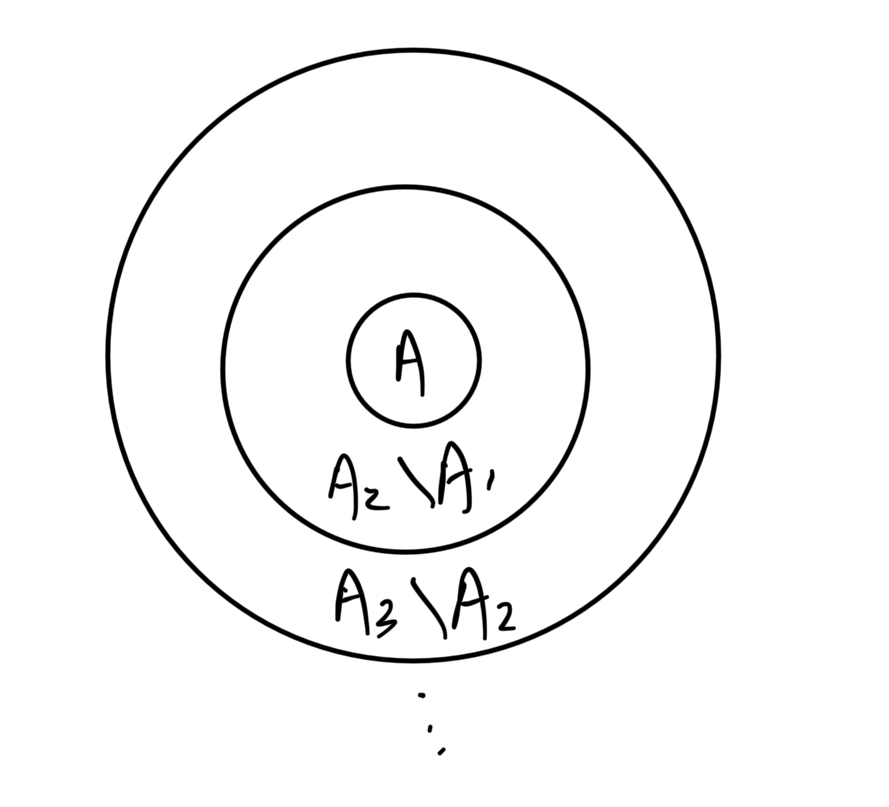
\includegraphics[width = 0.25 \linewidth]{images/1.jpeg} 
\end{figure}
Let $B_n = A_n \backslash A_{n-1}$, $A_0 = \phi$
\begin{align*}
\mathbb{P}(\lim _{n \rightarrow \infty} A_n) &= \mathbb{P} (\bigcup _{n=1}^{\infty} A_n)\\
&= \mathbb{P}(\bigcup _{n=1}^{\infty} B_n)\\
&= \sum_{n=1}^{\infty} \mathbb{P}(B_n) \text{ (countable additivity)}\\
&= \lim _{N \rightarrow \infty} \sum_{n=1}^{N} \mathbb{P}(B_n) \\
&= \lim _{N \rightarrow \infty} \mathbb{P}(\bigcup _{n=1}^{N} B_n)\\
&= \lim _{N \rightarrow \infty} \mathbb{P}(A_n)
\end{align*}
\end{enumerate}
\newpage

\section{Probability Generating function}
\begin{enumerate}
\item Definition: generating function\\
Let's say we have a sequence $a_i = \{a_0, a_1,a_2, ...\}$, we can define a generating function $G_a(s)$ for $a_i$.\\
$$G_a(s)=\sum_{i=0}^{\infty}a_{i} s^{i}$$
We could get back $a_{i}$ from $G_{a}(s)$ \textbf{in most but not all cases} (only when the derivatives and countable sum are inter-changable).
$$a_{i} = \dfrac{G_{a}^{(i)}(0)}{i!} $$
counter-example: \\
$$a_1 = \sin{nx} \text{, } a_n = \dfrac{\sin{nx}}{n} - \dfrac{\sin{(n-1)x}}{n-1} \text{ for $n = 2,3,...$}$$ \\

\item Convolution \\
Suppose we have two sequence $a_i$, $b_i$,
$$a_i = \{a_0, a_1, a_2, ... \}, b_i = \{b_0, b_1, b_2, ... \}$$
we then define another sequence $c_i$,
$$c_n = a_{n} * b_{n} = \sum_{i=0}^{n} a_i b_{n-i}$$
$$c_i=\{a_{0}b_{n}, a_{0}b_{n}+a_{1}b_{n-1}, a_{0}b_{n}+a_{1}b_{n-1}+a_{2}b_{n-2}\}$$
Then , we claim that $G_{c}(s) = G_{a}(s)G_{b}(s)$.\\
\textit{Proof}:
\begin{align*}
G_{c}(s) &= \sum_{i=0}^{\infty} c_{n} s^{n}\\
&= \sum_{n=0}^{\infty} \sum_{i=0}^{n} a_i b_{n-i} s^{n}\\
&= \sum_{n=0}^{\infty} \sum_{i=0}^{n} a_i b_{n-i} s^{i} s^{n-i} \\
&= \sum_{i=0}^{\infty} \sum_{n=i}^{\infty} a_i b_{n-i} s^{i} s^{n-i} \\
&= \sum_{i=0}^{\infty} a_{i} s^{i} \sum_{n=i}^{\infty} b_{n-i} s^{n-i} \\
&= \sum_{i=0}^{\infty} a_{i} s^{i} \sum_{n-i=0}^{\infty} b_{n-i} s^{n-i} \\
&= \sum_{i=0}^{\infty} a_{i} s^{i} \sum_{j=0}^{\infty} b_{j} s^{j}  = G_{a}(s) G_{b}(s)\\
\end{align*}

\item Definition: Probability Generating Function\\
The probability generating function of a discrete random variable $X$ taking non-negative integer value is given by
$$G_{X}(s) = \mathbb{E}(s^{X})= \sum_{i=0}^{\infty}f_{X}(i) s^{i}$$
\textit{Power series (review of calculus II)}\\
Let's say we a power series $f(s) = \sum_{n=0}^{\infty}a_n s^n$, how to find its radius of convergence $R$?
\begin{enumerate}
\item use root test (definition)
\begin{align*}
\lim_{n \to \infty} \sqrt[n]{|a_n s^{n}|} &<1\\
\lim_{n \to \infty} \sqrt[n]{|a_n|}|s| &<1\\
|s| &= \dfrac{1}{\lim_{n \to \infty} \sqrt[n]{|a_n|}} := R
\end{align*}
\item use ratio test (informal)
\begin{align*}
\lim_{n \to \infty} |\dfrac{a_{n+1}s^{n+1}}{a_{n}s^{n}}| &<1\\
\lim_{n \to \infty} |\dfrac{a_{n+1}}{a_{n}}||s| &<1\\
|s| &< \dfrac{1}{\lim_{n \to \infty} |\dfrac{a_{n+1}}{a_{n}}|} := R
\end{align*}
\end{enumerate}
\textit{Theorem}
If $R$ is the radius of convergence of $G_{a}(s) = \sum_{n=0}^{\infty}a_n s^{n}$, then
\begin{enumerate}
\item $G_a(s)$ converges absolutely  for all $|s|<R$ and diverges for all $|s|>R$.
\item for $|s|<R$, $G_a(s)$ is differentiable or integratable for any fixed number of times term by term (i.e. derivative and countable summation is interchangable).
\item for $R \neq 0$, and $G_a(s) = G_b(s)$ for $|s|< R'$ for some $0<R'<R$, then $a_n = b_n$ for all $n$.
\end{enumerate}
\textit{Question} Why do we care about $s = 1$?\\
Because we can find the moment $\mathbb{E}X$ using $G_{X}'(1)$, however, (b) in above theorem haven't cover the case when $s =1$. (we still don't know if we can inter-change derivative and countable summation when $s<R =1$)\\
This could be solved by applying abel theorem as following.

\item Abel Theorem\\
If $a_n \geq 0\,\, \forall n$, $G_a(s)$ is its generating function having the radius of convergence $R =1$, then additionally if $\sum_{n=0}^{\infty}a_n$ converges in $\mathbb{R} \cup \{\infty\}$, then we have 
$$\lim_{s \to 1^{-}} G_{a}(s) = \lim_{s \to 1^{-}} \sum_{n=0}^{\infty} a_n s^n = \sum_{n=0}^{\infty}a_n \lim_{s \to 1^{-}} s^{n} = \sum_{n=0}^{\infty}a_n$$

\item Probability generating functions of some typical random variables\\
\begin{tabular}{|c|p{6cm}|p{6cm}|}
\hline
Random variables& Generating functions& interval of $s$\\
\hline
$Be(p)$& $G_{X}(s) = 1-p + ps$& $\mathbb{R}$\\
\hline
$Bin(p)$& $G_{X}(s) = (1-p + ps)^n$& $\mathbb{R}$\\
\hline
$Poisson(\lambda)$& $G_{X}(s) = e^{\lambda (s-1)}$& $\mathbb{R}$\\
\hline
$Geom(p)$& $G_{X}(s) = \frac{ps}{1-s(1-p)}$& $|s| < \frac{1}{1-p}$\\
\hline
\end{tabular}

\item Moment and probability generating functions\\
If $X$ has probability generating function $G_{X}(s)$ then
\begin{enumerate}
\item $\mathbb{E}X = \lim_{s \to 1^{-}}G'(s) := G'(1)$
\item $\mathbb{E}[X(X-1)(X-2)...(X-(k-1))]=\mathbb{E}\frac{X!}{(X-k)!}= \lim_{s \to 1^{-}}G^{k}(s):= G^{k}(1)$
\end{enumerate}
\textit{Remark}
\begin{align*}
Var(X) &= \mathbb{E}X^2 - (\mathbb{E}X)^2\\
&= \mathbb{E}X(X-1) + \mathbb{E}(X)-(\mathbb{E}X)^2\\
&= G''(1) + G'(1) -(G'(1))^2
\end{align*}

\item Sum of independent random variables\\
\textit{Theorem} if $X \indep Y$, then $G_{X+Y}(s)= G_{X}(s)G_Y(s)$\\
\textit{Proof} 
\begin{align*}
f_{X+Y}(z) &= f_{X}*f_{Y}(z) = \sum_{x=0}^{z} f_{X}(x)f_{Y}(n-x)\\
G_{X+Y}(z) &= \sum_{n=0}^{\infty}f_{X+Y}(z)z^{n} \\
&= \sum_{n=0}^{\infty}\sum_{x=0}^{z} f_{X}(x)f_{Y}(n-x)z^{x} z^{n-x}\\
&= \sum_{x=0}^{\infty}\sum_{z=x}^{\infty} f_{X}(x)f_{Y}(n-x)z^{x} z^{n-x}\\
&= \sum_{x=0}^{\infty}f_{X}(x)z^{x} \sum_{z=x}^{\infty} f_{Y}(n-x) z^{n-x}\\
&= G_{x}(z) G_{Y}(z)
\end{align*}
\textbf{Caution: its converse may not be true!}

\item Sum of random number of random variables\\
\textit{Theorem}\\
 If $X_1, X_2, X_3, ..., X_N$ (i.i.d) with common probability generating function $G_X(s)$ and $N \geq 0$ is a random variable independent of all $X_i$'s with probability generating function $G_N(s)$. Let $$T = X_1 + X_2 +...+X_N$$, then $$G_{T}(s) = G_{N}(G_{X}(s))$$
 
 \textit{Proof}
 \begin{align*}
 G_{T}(s)&= \mathbb{E}s^{T}\\
 &= \mathbb{E}(\mathbb{E}(s^T |N))\\
 &= \sum_{n=0}^{\infty} \mathbb{E}(s^T |N=n) \mathbb{P}(N=n)\\
 &= \sum_{n=0}^{\infty} \mathbb{E}(s^{X_1 + X_2 +...+X_n}) \mathbb{P}(N=n)\\
 &= \sum_{n=0}^{\infty} (G_X(s))^n \mathbb{P}(N=n)\\
 &= G_{N}(G_X(s))
 \end{align*}
 
 \textit{Example} Sum of a Poisson number of independent Bernouli is still a Poisson.\\
 A hen lays $N$ eggs where $N \sim Poisson(\lambda)$. Each egg hatches with probability $p$ independently. Let $K$ be the number of chicks. Then, $$K = X_1 + X_2 + ...+X_N$$, where $X_i \sim Be(p)$ is the indicator random variable indicating where the $i$-th egg hatches or not, i.e.,$$X_i = 1, \text{if i-th egg hatches}, X_i = 0 \text{, otherwise}$$
 Therefore we can just apply the formula,
 \begin{align*}
 G_K(s) &= G_N(G_X(s))\\
 &= e^{\lambda (G_X(s) -1)}\\
 &= e^{\lambda (1-p+ps -1)}\\
  &= e^{\lambda p(1-s)}
 \end{align*}
Therefore, we could deduce that $K \sim Poisson(\lambda p)$

\item Multivariate extension: joint probability generating function
$$G_{X_1,X_2}(s_1, s_2) = \mathbb{E}{s_{1}}^{X_1}{s_{2}}^{X_2} = \sum_{i=0}^{\infty} \sum_{j=0}^{\infty} s_1 ^{i} s_2 ^{j} f_{X_1, X_2}(i, j)$$
$$f_{X_1, X_2}(i,j) = \dfrac{1}{i!j!} \dfrac{\partial^{i+j}}{\partial s_1 ^i \partial s_2 ^j}G_{X_1, X_2}(s_1, s_2)|_{(s_1,s_2)=(0,0)}$$
\textit{Theorem} $X_1 \indep X_2 \iff G_{X_1, X_2}(s_1, s_2)=G_{X_1}(s_1)G_{X_2}(s_2)$

\item Application 1: recurrence/ transience of 1D simple random walk \\
Let $S_n = \sum_{i=0}^{n} X_i$, $S_0 =0$, $n \geq 0$, where $S_n$ is the location at $n$-step, $X_i$ is representing the $i$-th step such that $\mathbb{P}(X_i =1)= p, \mathbb{P}(X_i = -1)= 1-p := q$.\\
Let $T_0 := \min \{i \geq 0 : S_{i} =0\}$, representing the first return time to the origin (i.e., how many steps to take for return to the origin?).\\\\
\textit{Remark} $Y$ is "defective" random variable $\iff$ $\mathbb{P}(Y = \infty) >0$ \newpage
\textit{Question} When is $T_0$ "defective"? It suffices to find $\mathbb{P}(T_0 = \infty)$ for different $p$ and $q$.\\
\textit{Solution}\\
Let $f_0 (n) := \mathbb{P}(S_1 \neq 0, S_2 \neq 0, S_3 \neq 0, ..., S_n = 0) = \mathbb{P}(T_0 =n)$ for $n \geq 1$.\\
Then, define its generating function $F_0(n)$
\begin{align*}
F_0(n) &= \sum_{n=1}^{\infty} f_0 (n) s^n\\
&= \lim_{N \to \infty} \sum_{n=1}^{N} f_0 (n) s^n\\
&\text{Since $\infty$ is not measured by the random variable $T_0$}\\
F_0(1) &= \lim_{N \to \infty} \sum_{n=1}^{N} f_0 (n) = 1 - \mathbb{P}(T_0 = \infty)
\end{align*}
Also, let $p_0 (n) = \mathbb{P}(S_n =0) = {{n} \choose {\frac{n}{2}}} p^{n/2} q^{n/2}$ for even $n$ and $p_0 (0) =  \mathbb{P}(S_0 =0) = 1$ since initial location is $0$.\\
Similarly, define its generating function $P_0(s) := \sum_{n=1}^{\infty} p_0 (n) s^n = (1-4pq s^2)^{-\frac{1}{2}}$ after some calculations\\
\textit{Theorem}
\begin{enumerate}
\item $P_0 (s) = 1+ P_0 (s)F_0 (s)$
\item $P_0 (s) = (1-4pq s^2)^{-1/2}$ (known)
\item $F_0 (s) = 1 - (1-4pq s^2)^{1/2}$ (easy by (a) and (b))
\end{enumerate}
\textit{Proof of (a)}\\
Let $A_n = \{S_{n} =0 \}$ (i.e., at $n$-th step, it returns to origin),\\
$B_{k} = \{S_1 \neq 0, S_2 \neq 0, ..., S_{k-1} \neq 0, S_{k} =0\}$ (i.e., at $k$-th step, it returns to origin first time).\\
Note that $p_0 (n) = \mathbb{P}(A_n)$, $f_0 (k) = \mathbb{P}(B_n)$.\\
By law of total probability,$$\mathbb{P}(A_n) = \sum_{k=1}^{n}\mathbb{P}(A_n | B_k) \mathbb{P}(B_k)$$
Let's consider 
\begin{align*}
\mathbb{P}(A_n | B_k) \mathbb{P}(B_k) &= \mathbb{P}(S_n =0 | S_1 =0 , S_2 =0, ..., S_k =0)\\
&= \mathbb{P}(S_n =0| S_k =0)\\
&= \mathbb{P}(S_{n-k} =0)\\
&= \mathbb{P}(A_{n-k})\\
&= p_0 (n-k)
\end{align*}
Therefore, we have 
\begin{align*}
p_0(n)&=\mathbb{P}(A_n)\\
 &= \sum_{k=1}^{n}\mathbb{P}(A_n | B_k) \mathbb{P}(B_k)\\
&= \sum_{k=1}^{n} p_0 (n-k) f_0(k),\text{ for } n >=1\\
p_o(0)&= 1
\end{align*}
As a result, we have
\begin{align*}
P_0(s) &= \sum_{n=0}^{\infty}p_0(n)s^{n}\\
&= p_0(0) + \sum_{n=1}^{\infty}\sum_{k=1}^{n} p_0 (n-k) f_0(k)s^{n}\\
&= 1 + \sum_{k=1}^{\infty} \sum_{n=k}^{\infty}  p_0 (n-k) f_0(k)s^{n}\\
&= 1 + \sum_{k=1}^{\infty} \sum_{n=k}^{\infty}  p_0 (n-k) f_0(k)s^{k}s^{n-k}\\
&= 1+ P_0(s)F_0(s)
\end{align*}
\textit{Conclusion}\\
\textbf{case 1}\\
If $p=q=\frac{1}{2}$, then $F_0(1)=1-(1-4(1/2)(1/2)(1)^2)^{1/2}=1$. Therefore, $\mathbb{P}(T_0 = \infty) = 1- F_0(1) =0$. In this case, we call this a recurrence since $T_0$ is not "defective".\\
\textbf{case 2}\\
If $p\neq q$, then $F_0(1) <1$. $\mathbb{P}(T_0 = \infty) > 0$. We call this a transient since $T_0$ is "defective".
\end{enumerate}
\newpage
\section{Characteristic Function}
\begin{enumerate}
\item{definition}: 
The characteristic function of a given random variable $X$ is given by $$\phi _{X} (t) = \mathbb{E}(e^{itX})= \int_{-\infty}^{\infty}e^{itx} f_{X}(x) dx = \int_{-\infty}^{\infty} \cos{itx} f_{X}(x) dx + i\int_{-\infty}^{\infty} \sin{itx} f_{X}(x) dx$$
\end{enumerate}
\newpage

\section{Convergence of Random Variables}
\begin{enumerate}
\item{Modes of convergence of random variables}
\begin{enumerate}
\item{Almost surely convergence}
$$X_{n} \xrightarrow{a.s.} X \iff \mathbb{P}(\lim_{n \to \infty}X_{n} (\omega) \to X, \forall \omega \in \Omega) \iff \mathbb{P}(|X_{n} - X| \geq \epsilon, i.o.) = 0$$
\textit{Remark}: Almost surely convergence can be proved by B.C.I and disproved by B.C.II.
\item{Convergence in $r$th-mean}
$$X_{n} \xrightarrow{r} X \iff \mathbb{E}(|X_{n} - X|^{r}) \to 0, r \geq 1$$
Alternatively, we have proof $\mathbb{E}(|X_{n} - X|^{r})^{\frac{1}{r}} \to 0$.\\
\textit{Remark}:$X_{n} \xrightarrow{r} X \implies X_{n} \xrightarrow{l} X$ for $1\leq l < r$
\item{Convergence in probability}
$$X_{n} \xrightarrow{\mathbb{P}} X \iff \mathbb{P}(|X_{n} - X| \geq \epsilon) \to 0 $$
\item{Convergence in distribution}
$$X_{n} \xrightarrow{D} X \iff \mathbb{P}(X_{n} \leq x) \to \mathbb{P}(X \leq x)$$
\end{enumerate}
\item{Ways to proof convergences}
\begin{enumerate}
\item{Almost surely convergence}
\begin{enumerate}
\item{Directly show for 'almost' all $\omega$ in $\Omega$, $$\mathbb{P}(\lim_{n \to \infty} X_{n}(\omega) = X(\omega)) = 1$$}
\item{(Seldom) Show $$\forall \epsilon > 0, \mathbb{P}(\lim_{n \to \infty}|X_{n} - X| < \epsilon) = 1$$} 
\item{Use Borel-Cantelli Lemma I}\\
Show that $$\forall \epsilon > 0, \sum_{n=1}^{\infty}\mathbb{P}(|X_{n} - X|> \epsilon)< \infty$$, then we can apply B.C. I to show that 
$$\mathbb{P}(\limsup_{n \to \infty} |X_{n} - X|> \epsilon) = 0$$
\item{(As complement of (iii))}\\
If we find  $\sum_{n=1}^{\infty}\mathbb{P}(|X_{n} - X|> \epsilon)= \infty$,\\
show that for $\epsilon>0$,  $\text{let }B_{n} = \{|X_{n} - X| < \epsilon \}$,
$$X_{n} \xrightarrow{a.s.} X \iff \lim_{n \to \infty} \mathbb{P}(\bigcap_{m=n}^{\infty}B_{m})=1$$
\textit{Proof}:\\
For all $\epsilon > 0$, let $A_{n} = \{|X_{n} - X| \geq \epsilon\}$.
\begin{align*}
X_{n} \xrightarrow{a.s.} X &\iff \mathbb{P}(A_{n}, i.o.) = 0\\
&\iff \mathbb{P}(\bigcap_{m=1}^{\infty} \bigcup_{n=m}^{\infty} A_{n}) = 0\\
&\iff \mathbb{P}((\bigcap_{m=1}^{\infty} \bigcup_{n=m}^{\infty} A_{n})^{c}) = 1\\
&\iff \mathbb{P}(\bigcup_{m=1}^{\infty} \bigcap_{n=m}^{\infty} A_{n}^{c}) = 1\\
&\iff \lim_{n \to \infty} \mathbb{P}(\bigcap_{n=m}^{\infty} A_{n}^{c}) =1\\
&\iff \lim_{n \to \infty} \mathbb{P}(\bigcap_{n=m}^{\infty} B_{n}) =1 &(B_{n} := A_{n}^{c})
\end{align*}
\textit{Remark:} If $X_{i}$'s are independent, then $$X_{n} \xrightarrow{a.s.} X  \iff \lim_{n \to \infty} \prod_{n=m}^{\infty} \mathbb{P}(B_{n}) =1$$
\end{enumerate}
\item{Convergence in $r$-th mean}
\begin{enumerate}
\item{Directly show $\lim_{n \to \infty} \mathbb{E}|X_{n} - X|^{r} = 0$ or $\lim_{n \to \infty}(\mathbb{E}|X_{n}-X|^{r})^{\frac{1}{r}} = 0$}
\item{Useful formulas}
\begin{enumerate}
\item[•]{Triangular inequality}
$$(\mathbb{E}|X_{n}|^{r})^{\frac{1}{r}} = (\mathbb{E}|X_{n} - X + X|^{r})^{\frac{1}{r}} \leq (\mathbb{E}|X_{n} -X|^{r})^{\frac{1}{r}}+(\mathbb{E}|X|^{r})^{\frac{1}{r}}$$
$$\iff (\mathbb{E}|X_{n}|^{r})^{\frac{1}{r}} - (\mathbb{E}|X|^{r})^{\frac{1}{r}} \leq (\mathbb{E}|X_{n} -X|^{r})^{\frac{1}{r}}$$
\item[•]{Hölder's inequality}\\
For $1 < p, q < \infty, \dfrac{1}{p} + \dfrac{1}{q} = 1$,
$$\mathbb{E}|XY| \leq (\mathbb{E}|X|^{p})^{\frac{1}{p}} (\mathbb{E}|X|^{q})^{\frac{1}{q}}$$
\end{enumerate}
\end{enumerate}
\item{Convergence in probability}
\begin{enumerate}
\item{Directly show for all $\epsilon > 0$, $\lim_{n \to \infty}\mathbb{P}(|X_{n} - X| \geq \epsilon) = 0$ or $\lim_{n \to \infty}\mathbb{P}(|X_{n} - X| < \epsilon) = 1$}
\item{(Partial converse theorem) Show that $X_{n} \xrightarrow{D} c$ which implies $X \xrightarrow{P} c$}.\\
\textit{Proof:}\\
Suppose $X_{n} \xrightarrow{D} c$, then for all $\epsilon >0$, $\lim_{n \to \infty} F_{X_n}(c - \epsilon) = 0$ and $\lim_{n \to \infty} F_{X_n}(c + \epsilon) = 1$.
\begin{align*}
\lim_{n \to \infty} \mathbb{P}(|X_{n} - c| \geq \epsilon) &= \lim_{n \to \infty} \mathbb{P}(X_{n} - c \geq \epsilon) + \lim_{n \to \infty}\mathbb{P}(X_{n} - c \leq -\epsilon)\\
&= \lim_{n \to \infty} \mathbb{P}(X_{n} \geq \epsilon + c) + \lim_{n \to \infty} \mathbb{P}(X_{n} \leq -\epsilon +c)\\
&= \lim_{n \to \infty} (1 - \mathbb{P}(X_{n} < \epsilon + c)) + \lim_{n \to \infty} \mathbb{P}(X_{n} \leq -\epsilon +c)\\
&= \lim_{n \to \infty} (1 - F_{X_n}(c + \epsilon)) + \lim_{n \to \infty} F_{X_n}(c - \epsilon)\\
&= (1 -1) +0\\
&= 0
\end{align*}
Thus, $X \xrightarrow{P} c$.
\item{Useful properties}
\begin{enumerate}
\item[•]{If $\omega \in A \implies \omega \in B$, then}
$$\mathbb{P}(A) \subseteq \mathbb{P}(B)$$
\item[•]{Triangular inequality}\\
$|X+Y| \leq |X| + |Y|$, \\$|X|= |X-Y+Y| \leq |X-Y|+|Y|$
\item[•]{Markov's inequality}\\
$$\mathbb{P}(X \geq \epsilon) \leq \dfrac{\mathbb{E}(g(X))}{g(\epsilon)}$$
\end{enumerate}
\end{enumerate}
\item{Convergence in distribution}
\begin{enumerate}
\item{Directly show $\lim_{n \to \infty} \mathbb{P}(X_{n} \leq x) = \lim_{n \to \infty} \mathbb{P}(X \leq x)$}
\item{For non-negative integer valued discrete random variables}\\
If $X_{1}, X_{2}, X_{3}, ...$ are non-negative integer valued random variables, then $$X_{n} \xrightarrow{D} X \iff \lim_{n \to \infty} \mathbb{P}(X_{n} = x) = \mathbb{P}(X = x)$$
\textit{Proof:}
\begin{enumerate}
\item{Proving $X_{n} \xrightarrow{D} X \implies \lim_{n \to \infty} \mathbb{P}(X_{n} = x) = \mathbb{P}(X = x)$}\\
Suppose $X_{n} \xrightarrow{D} X \implies \lim_{n \to \infty} F_{X_{n}}(x) = F_{X}(x)$,\\
Note: since $X_{n}$'s are non-negative valued, then $F_{X_{n} (x)}$ is continuous in $x \in \mathbb{R} \backslash \{0, 1,2,3, ... \}$.
\begin{align*}
\lim_{n \to \infty} \mathbb{P}(X_{n} = x) &= \lim_{n \to \infty} (\mathbb{P}(X_{n} = x+ \frac{1}{2}) - \mathbb{P}(X_{n} = x- \frac{1}{2}))\\
&=\lim_{n \to \infty}F_{X_{n}}(x + \frac{1}{2}) - \lim_{n \to \infty}F_{X_{n}}(x - \frac{1}{2})\\
&=F_{X}(x + \frac{1}{2}) - F_{X}(x - \frac{1}{2})\\
&= \mathbb{P}(X = x)
\end{align*}
Thus, $\lim_{n \to \infty} \mathbb{P}(X_{n} = x) = \mathbb{P}(X = x)$.
\item{Proving $\lim_{n \to \infty} \mathbb{P}(X_{n} = x) = \mathbb{P}(X = x)\implies X_{n} \xrightarrow{D} X$}\\
Suppose $\lim_{n \to \infty} \mathbb{P}(X_{n} = x) = \mathbb{P}(X = x)$,
\begin{align*}
\lim_{n \to \infty} F_{X_{n}}(x) &= \lim_{n \to \infty} \mathbb{P}(X_{n} \leq x)\\
&= \lim_{n \to \infty} \sum_{i=0}^{\lfloor \frac{1}{x} \rfloor} \mathbb{P}(X_{n} = i)\\
&= \sum_{i=0}^{\lfloor \frac{1}{x} \rfloor} \mathbb{P}(X = x)\\
&= \mathbb{P}(X \leq x)\\
&= F_{X}(x)
\end{align*}
Thus, we have $X_{n} \xrightarrow{D} X$.
\end{enumerate}
\end{enumerate}
\end{enumerate}
\item{Relationships between modes of convergence}
\begin{enumerate}
\item{$X_{n} \xrightarrow{a.s.} X \implies X_{n} \xrightarrow{\mathbb{P}} X$}
\item{$X_{n} \xrightarrow{r} X \implies X_{n} \xrightarrow{\mathbb{P}} X$}
\item{$X_{n} \xrightarrow{\mathbb{P}} X \implies X_{n} \xrightarrow{D} X$}
\end{enumerate}
\item{Borel-Cantelli Lemma}\\
Let's say $A_n$ is a sequence of event in $\mathcal{F}$.
\begin{enumerate}
\item{B.C. I}\\ 
If $\sum_{n=1}^{\infty}\mathbb{P}(A_n) < \infty$,  then $\mathbb{P}(\limsup_{n \to \infty} A_n) = 0$.\\
\textit{Proof:} \begin{align*}
\mathbb{P}(\limsup_{n \to \infty} A_n) &= \mathbb{P}(\bigcap_{n=1}^{\infty} \bigcup_{m=n}^{\infty}A_m)\\
&= \lim_{n \to \infty} \mathbb{P}(\bigcup_{m=n}^{\infty}A_m)\\
&\leq \lim_{n \to \infty} \sum_{m=n}^{\infty} \mathbb{P}(A_n)\\
&=0 &\text{(by the assumption in the if statement)}
\end{align*}
\item{B.C. II}\\
If $\sum_{n=1}^{\infty}\mathbb{P}(A_n) = \infty$ and $A_n$'s are independent, then $\mathbb{P}(\limsup_{n \to \infty}) = 1$.\\
\textit{proof}: \\
We want to show that $\mathbb{P}(\limsup_{n \to \infty} A_n) = 1$.\\This is same as showing that 
\begin{align*}
\mathbb{P}((\limsup_{n \to \infty} A_n)^{c}) &= \mathbb{P}((\bigcap_{n=1}^{\infty} \bigcup_{m=n}^{\infty}A_m)^{c})\\
&= \mathbb{P}(\bigcup_{n=1}^{\infty}\bigcap_{m=n}^{\infty} A_n ^c)\\
&= \lim_{m \to \infty} \mathbb{P}(\bigcap_{n=m}^{\infty} A_n ^c)\\
&= \lim_{m \to \infty} \lim_{r \to \infty} \mathbb{P} (\bigcap_{n=m}^{r} A_n ^c)\\
&= \lim_{m \to \infty} \lim_{r \to \infty} \prod_{n=m}^{r} \mathbb{P} (A_n ^c) \text{ (since $A_n$'s are independent)}\\
&= \lim_{m \to \infty} \lim_{r \to \infty} \prod_{n=m}^{r} (1-\mathbb{P} (A_n))\\
&\leq \lim_{m \to \infty} \prod_{n=m}^{\infty} e^{-\mathbb{P} (A_n)}\\
&= \lim_{m \to \infty} e^{\sum_{n=m}^{\infty} \mathbb{P}(A_n)}\\
&= \lim_{m \to \infty} e^{-\infty}\\
&= 0
\end{align*}
\end{enumerate}
\textit{Remark:} B.C. II is a partial converse statement of B.C. I.

\item{Different versions of Law of Large Numbers}
\begin{enumerate}
\item{WLLN}\\
If we have a sequence of random variables $X_1 , X_2, ...$ (i.i.d.), with $\mathbb{E}(X_1) = \mu < \infty$, then let $$S_{n} =  X_1 + X_2 + ... + X_{n} = \sum_{i =1}^{n} X_{i}$$
By WLLN, we have $$\frac{S_{n}}{n} \xrightarrow{D/ \mathbb{P}} \mu$$\\
\item{$L^{2}$-WLLN}\\
If we have a sequence of random variables $X_1 , X_2, ...$ where $X_{i}$'s are uncorrelated with $\mathbb{E}(X_{i}) = \mu$ \textit{(common mean)}, $Var(X_{i}) \leq c < \infty$ \textit{(bound variance)} for all $i$, then let $$S_{n} =  X_1 + X_2 + ... + X_{n} = \sum_{i =1}^{n} X_{i}$$
By $L^{2}$-WLLN, we have $$\frac{S_{n}}{n} \xrightarrow{2} \mu$$
\item{SLLN}\\
If we have a sequence of random variables $X_1 , X_2, ...$ (i.i.d.), with $\mathbb{E}(X_1) = \mu$ and $\mathbb{E}(|X_1 |) < \infty$, then let $$S_{n} =  X_1 + X_2 + ... + X_{n} = \sum_{i =1}^{n} X_{i}$$
By SLLN, $$\frac{S_{n}}{n} \xrightarrow{a.s.} \mu$$
\end{enumerate}
\end{enumerate}
\end{document}